\documentclass[a4paper]{article}
\usepackage[brazilian]{babel}
\usepackage{subfig}
\usepackage{booktabs}
\usepackage{graphicx}
\usepackage{listings}
\usepackage{hyperref}  
\usepackage{url}  
%-----------------------------------------------------------------
\title{Projeto computacional: Implementa\c{c}\~ao do algor\'itmo simplex}
\author{122830 Alcides Goldoni Junior\\
		148585 Guilherme de Freitas Laranja\\
		150946 Isabela Marton\\
	\small MS 428 - Programa\c{c}\~ao Linear\\
	}%Fechando Title
\begin{document}
\maketitle
%--------------------------------------------------------------------------------------------------
%Seções
%--------------------------------------------------------------------------------------------------
\section{Introdu\c{c}\~ao}

O m\'etodo simplex \'e uma ferramenta utilizada para encontrar o conjunto de solu\c{c}\~oes \'otimas para problemas de otimiza\c{c}\~ao linear.

Esse m\'etodo viabiliza a solu\c{c}\~ao de muitos problemas de programa\c{c}\~ao linear e \'e muito popular.

Ele permite que se encontre valores ideais em situa\c{c}\~oes em que condi\c{c}\~oes necessitam ser respeitadas.

%--------------------------------------------------------------------------------------------------
\section{Funcionamento}
Para o funcionamento da biblioteca simplex desenvolvida \'e preciso ter as bibliotecas gsl (GNU Scientific Library) eliblapack instaladas. Essas bibliotecas ajudam nas opera\c{c}\~oes envolvendo vetores e matrizes, e tamb\'em na resolu\c{c}\~ao dos sistemas lineares presentes no algor\'itmo Simplex.

Para a instala\c{c}\~ao Linux (Debian Like):
\begin{lstlisting}[language=bash]
  # apt-get install libgsl-dev liblapack-dev
\end{lstlisting}

Para a instala\c{c}\~ao MacOS:
\begin{lstlisting}[language=bash]
  # brew install gsl 
\end{lstlisting}

Para compilar o programa, utiliza-se os arquivos compile.bash ou compileLinux.bash (para MacOS e Linux, respectivamente).

Linux:
\begin{lstlisting}[language=bash]
  # ./compileLinux.bash 
\end{lstlisting}

MacOS:
\begin{lstlisting}[language=bash]
  # ./compile.bash 
\end{lstlisting}

Ser\'a gerado um bin\'ario de nome "simplexExec" respons\'avel pela executa\c{c}\~ao do programa.

A melhor forma de executar o programa \'e editar o arquivo teste.in onde cada linha representa uma entrada:

\begin{itemize}
\item Linha 1: N\'umero de restri\c{c}\~oes (linhas) e n\'umero de vari\'aveis (colunas),
\item Linha 2: Vetor de custos da fun\c{c}\~ao objetivo,
\item Linha 3: Vetor de recursos
\item As pr\'oximas linhas respresentam a matriz dos coeficientes de restri\c{c}\~ao.
\end{itemize}

Dessa forma, o arquivo teste.in ficar\'a da seguinte forma:

\begin{lstlisting}[language=bash]
 2 5
 1 2 3 4 5
 2 2
 7 5 3 1 0
 6 4 2 0 1
\end{lstlisting}

Para a execu\c{c}\~ao:

\begin{lstlisting}[language=bash]
  # ./simplexExec < teste.in
\end{lstlisting}

Caso n\~ao queira editar o arquivo, pode-se digitar as entradas baseadas na perguntas que o pr\'oprio programa pede. Neste caso, para a execu\c{c}\~ao do programa fica da seguinte forma:

\begin{lstlisting}[language=bash]
  # ./simplexExec 
\end{lstlisting}

A imagem a seguir, ilustra a execu\c{c}\~ao e as entradas para o programa:

\begin{figure}[ht!]
\caption{Exemplo para entradas do Simplex}
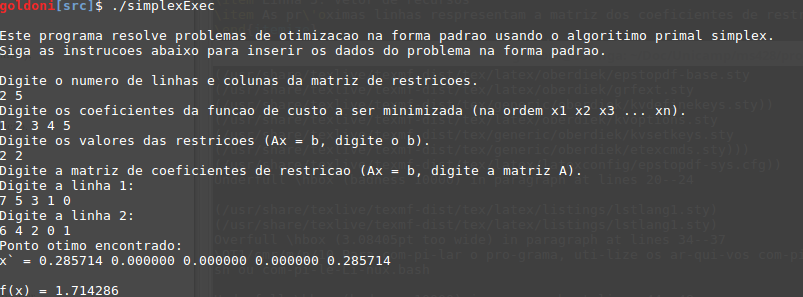
\includegraphics[width=0.95\textwidth]{simplexEntradas.png}
\end{figure}

Como sa\'ida, o programa retorna:

\begin{itemize}
\item O ponto encontrado e o valor da fun\c{c}\~ao, caso encontre a solu\c{c}\~ao;
\item A seguinte frase: "Problema infactivel!!! Ainda existem variaveis artificiais diferentes de zero na solucao encontrada com BigM", caso o problema n\~ao encontre solu\c{c}\~ao fact\'ivel;
\item A seguinte frase: "Problema nao tem solucao finita!!", caso o problema tenha infin\'itas solu\c{c}\~oes.
\end{itemize}
%--------------------------------------------------------------------------------------------------
\section{Testes}
Foram realizados tr\^es testes para validar o programa (fact\'ivel, infact\'ivel e ilimitado), cobrindo as poss\'iveis sa\'idas descritas anteriormente.
\begin{itemize}
\item Fact\'ivel:
\\
O seguinte exemplo (Figura 2) possui solu\c{c}\~ao fact\'ivel:
\\
Linhas: 2
\\
Colunas: 4
\\
Fun\c{c}\~ao: -$x_1$ - 3$x_2$ + 0$x_3$ + 0$x_4$
\\
Vetor b = [6 3]
\\
Matriz de restri\c{c}\~ao:\\
1 1 1 0\\
0 1 0 1\\
\begin{figure}[ht!]
\label{factivel}
\caption{Exemplo Simplex: Problema fact\'ivel}
\includegraphics[width=0.95\textwidth]{factivel.png}
\end{figure}
\\
\item Infact\'ivel
\\
O seguinte exemplo (Fingura 3) possui solu\c{c}\~ao infact\'ivel:
\\
Linhas: 2
\\
Colunas: 4
\\
Fun\c{c}\~ao: 2$x_1$ + 2$x_2$ + 0$x_3$ + 0$x_4$
\\
Vetor b = [1 -1]
\\
Matriz de restri\c{c}\~ao:\\
-1 1 -1 0\\
1 1 0 1\\
\begin{figure}[h!]
\label{infactivel}
\caption{Exemplo Simplex: Problema infact\'ivel}
\includegraphics[width=0.95\textwidth]{infactivel.png}
\end{figure}
\item Ilimitado
\\
O seguinte exemplo (Fingura 4) possui solu\c{c}\~ao infact\'ivel:
\\
Linhas: 2
\\
Colunas: 4
\\
Fun\c{c}\~ao: $x_1$ + $x_2$ + 0$x_3$ + 0$x_4$
\\
Vetor b = [1 2]
\\
Matriz de restri\c{c}\~ao:\\
1 1 -1 0\\
1 1 0 -1\\
\begin{figure}[h!]
\label{ilimitado}
\caption{Exemplo Simplex: Problema ilimitado}
\includegraphics[width=0.95\textwidth]{ilimitado.png}
\end{figure}

\end{itemize}
\section{Discus\~ao}
Podemos ver que o programa se comportou como o esperado para os casos de solu\c{c}\~ao fact\'ivel e infact\'ivel, por\'em, para os casos de solu\c{c}\~ao ilimitada, ele n\~ao retorna o valor esperado. Investigamos por\'em n\~ao encontramos o mot\'ivo desse problema.

\section{Conclus\~ao}
Neste trabalho desenvolvemos o algor\'itmo Simplex em linguagem C e ultilizamos algumas bibliotecas j\'a prontas e conhecidas para facilitar sua escrita. 

Foi importante para consolidar o algorit\'imo visto em aula. 

O programa foi testados para  os poss\'iveis casos de uso por\'em s\'o foi bem sucedido nas situa\c{c}\~oes onde o problema era fact\'ivel ou infact\'ivel.
\end{document} 
